%The algorithms for the trigger
\section{Jet Algorithm for the Level 1 trigger upgrade}
To make use of the L1 trigger upgrades new algorithms must be developed that improve the identification of different particles. With more information available, it is possible to develop more efficient triggers for the various analyses carried out at CMS. The increase in granularity allows the trigger to have a better view of the substructure of energy deposits, allowing the identification of 3 pronged tau jets and isolated electrons that have varying deposits in the ECAL and HCAL for example. 
\\\\
One particular area of potential improvement is in the jet algorithm. During Run 1, the jet candidates were created from a $3\times3$ RCT region sliding window. Candidates in which the central region has the maximum energy are kept as jets. The performance of this algorithm will be severely reduced by the conditions that will be experienced during Run 2. The doubling of the LHC luminosity will result in $\sim$40 instantaneous collisions, or pileup (PU), per bunch crossing. In any bunch crossing with hard scattering event, it is likely that all other simultaneous collisions consist of soft QCD processes, and should therefore be ignored. The process to do this is known as pileup subtraction (PUS), and if done well should remove these soft processes and subtract the contribution they make to the hard physics process under consideration. With the coarse jets available at Run 1 and more limited hardware resources, correcting for the PU is difficult, as one does not want to subtract any interesting physics. The upgrade will therefore aim to carry out PUS and create a jet with a better position resolution.

\subsection{The Stage 2 Jet algorithm}
\label{sec:stage2_jetalgo}
The jet algorithm for Stage 2 of the CMS trigger upgrade operates on the TT-level calorimeter output, with the energy of each TT taken as the sum of the ECAL and HCAL energy. Each TT within $|\eta|<3$ is considered as a candidate. A $9\times9$ square of TTs with the candidate in the centre is constructed. The candidate is vetoed if any of the other TT in the square have an energy deposit of either greater than or greater than or equal to it. The veto condition applied is antisymmetric along the diagonal of the square to prevent TT with the same energy from vetoing one another. A representation of the square considered can be seen in Fig.~\ref{fig:stage2_jetalgo}(a). Any TT that pass this criteria are considered as jet centres, where the jet reconstructed from the TT has the energy equal to the sum of all the towers within the $9\times9$ square. 
\begin{figure}
	\begin{center}
		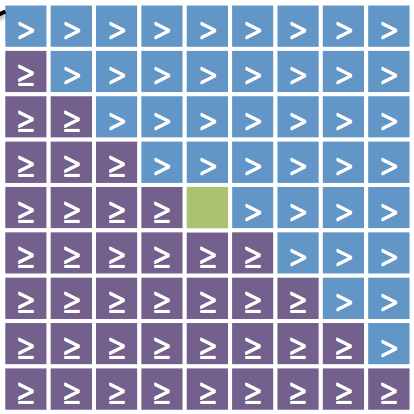
\includegraphics[width=0.3\linewidth]{stage2_jetalgo}\put(-32,143){(a)}
		\hspace{1cm}
		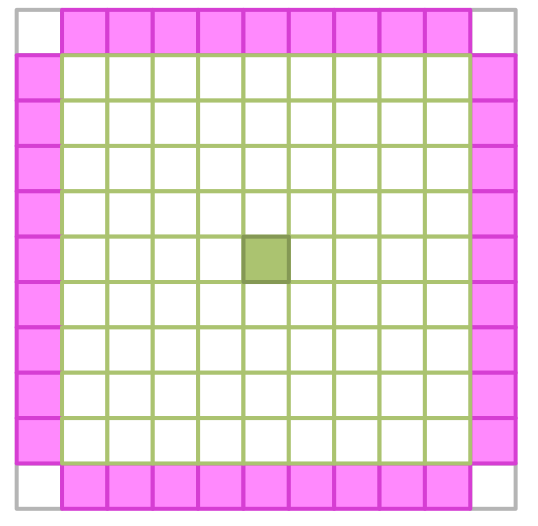
\includegraphics[width=0.3\linewidth]{Donut_plots/donut_region}\put(-32,143){(b)}
	\end{center}
	\caption{(a) The consideration of a Trigger Tower candidate for the Stage 2 Level 1 Trigger jet algorithm. The candidate (green) is vetoed if the energy of the other towers meets the condition shown in the blue and purple towers. (b) The ring considered around a jet when carrying out donut subtraction \cite{jad-l1jets}}
	\label{fig:stage2_jetalgo}
\end{figure}
\\\\
The motivation for the jets having a size of $9\times9$ TT is that the area of each jet is approximately equal to the maximum area allowed for offline jets that are reconstructed using the anti-kt with a maximum radius of 0.4 (AK4) \cite{antiktJetAlgorithm}. This is the algorithm that will be used for offline clustering during Run 2. Taking the highest energy TT as the centre of the jet axis is motivated by the fact that jets are boosted objects with most of their energy in the middle \cite{JetProfile_pileup}. The performance of the algorithm as compared to AK4 can be seen in Fig.~\ref{fig:ak4_comp}.
\begin{figure}
	\begin{center}
		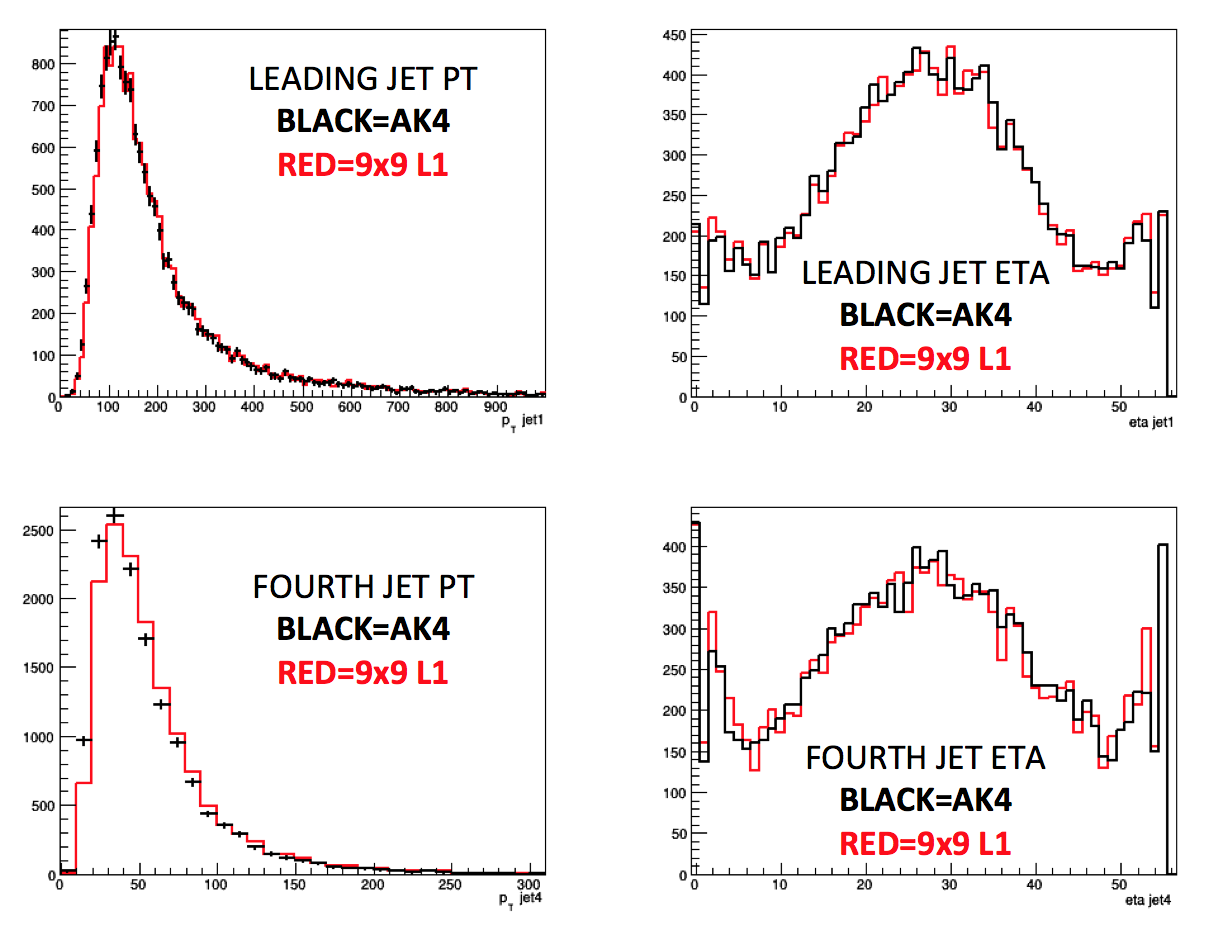
\includegraphics[width=0.8\linewidth]{jet_l1s2_compak4}
	\end{center}
	\caption{A comparison between the proposed Level 1 Stage 2 jet algorithm and anti-kt with R=0.4 with the Trigger Towers as input. These plots are produced from a $t\bar{t}$ Monte Carlo simulation at $13$~TeV with pileup $\sim40$ \cite{jad-l1jets}}
	\label{fig:ak4_comp}
\end{figure}
\\\\
The veto conditions applied on the central TT ensure that no two overlapping jets are reconstructed, avoiding the duplication of energy deposits. However, the algorithm can introduce inefficiencies in very specific jet topologies. In these cases a high energy TT vetoes a medium energy TT which then vetoes a lower energy TT. In this case the medium TT is included in the jet constructed by the high energy TT, however the lower energy TT is lost. This is not usually a problem from the L1 Trigger point of view, as the high energy TT will usually ensure that the event is triggered, despite energy being lost.

%Downsides-> fixed window -> lack of substructure (nsubjettyness)

\subsection{Pileup Subtraction Algorithms}
During or after the creation of L1 jets with the algorithm described in Section~\ref{sec:stage2_jetalgo}, PUS is performed. The purpose of this is to remove jets that originate from soft QCD scattering events and to correct the energy of jets from hard physics processes that have been contaminated by PU. The ideal scenario is one in which the energy of interesting jets is not dependent on the number of collisions during a bunch crossing. Three forms of PUS at L1 are outlined in here and investigated in Section~\ref{sec:jet_algo_performance}. These algorithms are designed to operate on an event-by-event basis, allowing the performance to change dynamically based on differing PU conditions. 
%cite global rho

\subsubsection{Global \boldmath $\rho$}
A prominent method of PUS is to find the average energy per unit area in the calorimeter due to PU, $\rho$, and subtract it from each reconstructed jet. A favoured estimator for this quantity is \cite{global_rho}:
\begin{equation}
\rho\equiv median(\frac{p_{Tj}}{A_j}),
\end{equation}
where $p_{Tj}$ is the transverse momentum of a jet $j$, $A_j$ is its area and the median is taken over all reconstructed jets in an event. This form of PUS is known as global $\rho$ and acts to remove the low energy half of jets in an event and correct the remaining high energy half. It works particularly well high PU cases as $\rho$ is insensitive to fluctuations in the energy of interesting physics events. 
\\\\
A disadvantage of global $\rho$ PUS is the fact that it is non local, it does not account for $\eta$ dependence of PU. In an ideal case PU on average has no $\eta$ dependence, although the response of the calorimeter trigger inputs is not fully independent. It is possible to calculate $\rho$ for particular ranges of $\eta$, local $\rho$, but this method loses robustness as the number of jets that are sampled is lowered for each $\rho$ calculation. 
%At L1, global $\rho$ subtraction also has a latency penalty in hardware, the jets must be found before it can be calculated and subtracted from their energies. Depending on available hardware resources this can present a problem.

\subsubsection{Seed Threshold}
A simple way of reducing the number of soft QCD jets is by introducing an energy threshold on the TT that can form a jet. The TT that is considered for a jet candidate in the algorithm outlined in Section~\ref{sec:stage2_jetalgo} is required to be above a certain energy, known as the seed threshold. This is very easy to implement in hardware, and has the potential to save latency as it reduces the number of jets that need to be made. A disadvantage is that it can kill soft jets that originate from a primary vertex. It is also not $\eta$ dependent, although this possibility is being investigated. For the following studies a seed of $2.5$~GeV (5 in L1 units) was chosen as a benchmark that appeared to kill PU jets without removing jets above 10~GeV from a zero PU $t\bar{t}$ test sample, the optimisation of this seed is to be studied. 

\subsubsection{Donut Subtraction}
The seed threshold does the job of removing PU jets, but does not correct the energy of the reconstructed high energy jets. As hard jets are boosted objects, it is assumed that they most of their energy is deposited very close to the central TT \cite{JetProfile_pileup}. Therefore, in the case of isolated jets, the ring $5$ TT from the centre of the jet can be assumed to contain only PU, see Figure~\ref{fig:stage2_jetalgo}(b). It is therefore proposed to take the energy per unit area in this ring, known as a donut, scale it up by the area of the jet and subtract the resulting energy from the jet. 
\\\\
This approach only works for correcting isolated jets, if one jet is in the vicinity of another the energy in the donut is inflated above that of PU as can be seen in Fig.~\ref{fig:donut_energies}(a). To mitigate this, only the median two $4\times1$ TT strips of the four that make up the donut are used to calculate the PU energy density. This lessens the effect of the contamination, shown in Fig.~\ref{fig:donut_energies}(b). To confirm that this final energy is a measure of the PU in the event, it is plotted against the number of interactions for a Monte Carlo (MC) simulation of $t\bar{t}$ 13~TeV data in Fig.~\ref{fig:donut_nint}. There is a good correlation, implying the donut energy should be a good measure of PU.
\\\\
%donut energy vs nint, response
\begin{figure}
	\begin{center}
		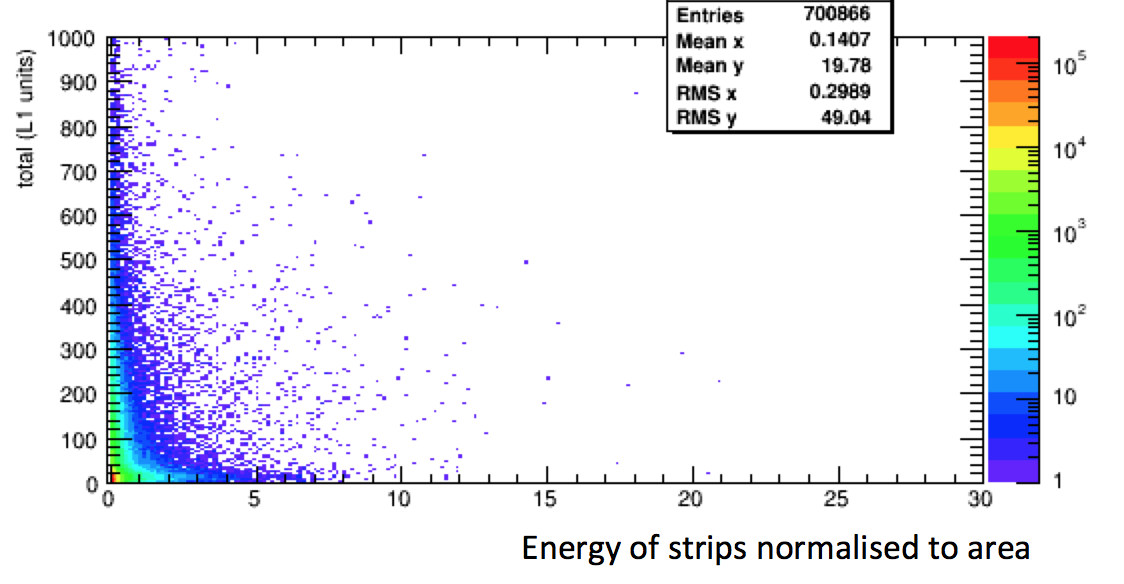
\includegraphics[width=0.5\linewidth]{Donut_plots/noniso_donut_energy}\put(-32,133){(a)}
		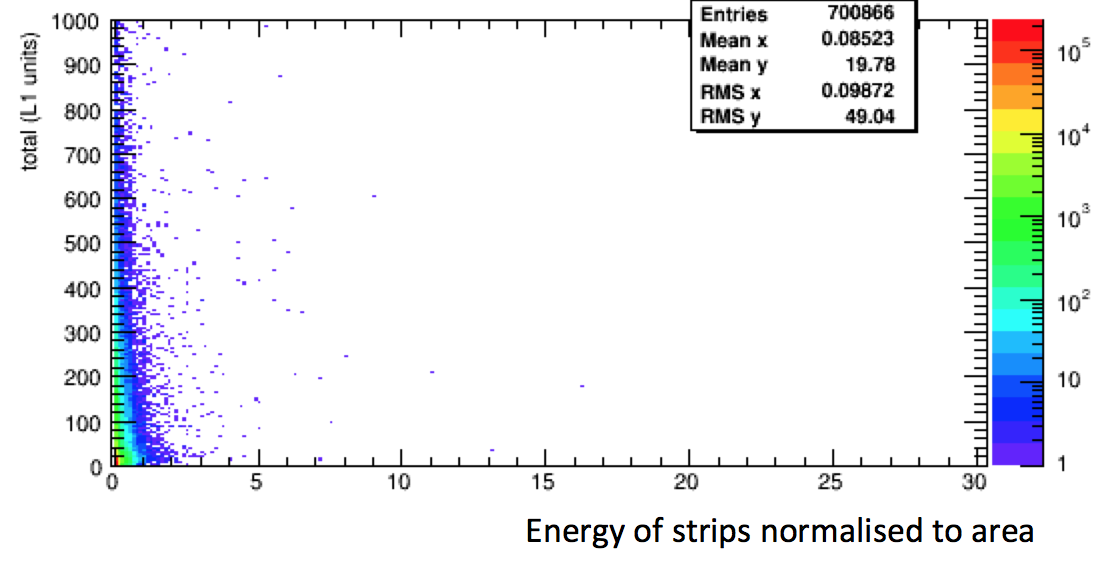
\includegraphics[width=0.5\linewidth]{Donut_plots/noniso_finaldonut_energy}\put(-32,133){(b)}
	\end{center}
	\caption{(a) The energy per unit area in units of $0.5$~GeV/TT of the donut ring taken around the jet. (b) The energy per unit area in units of $0.5$~GeV/TT of the median two strips of the donut ring taken around the jet}
	\label{fig:donut_energies}
\end{figure}
\begin{figure}
	\begin{center}
		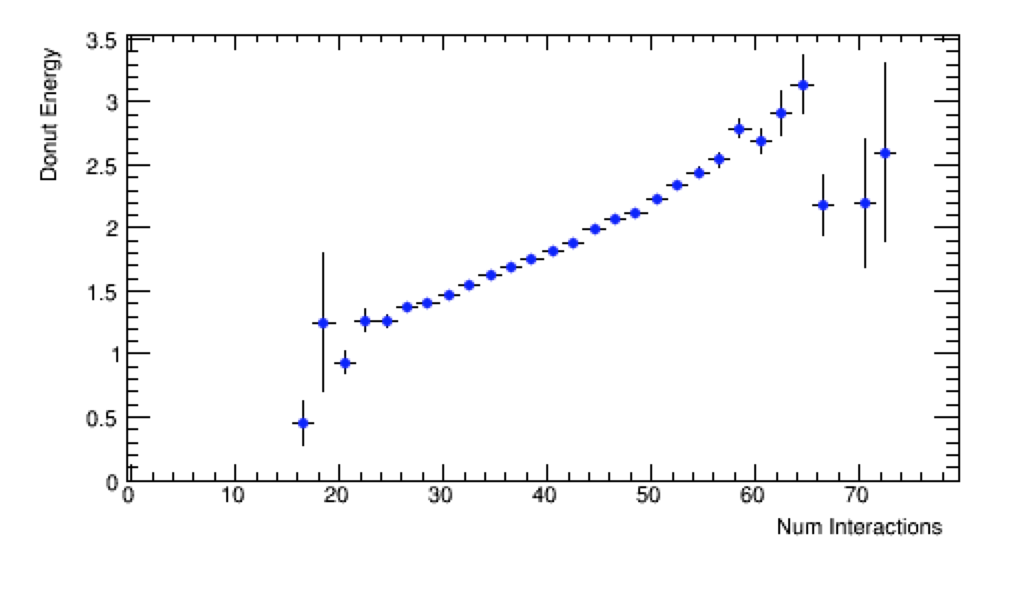
\includegraphics[width=0.6\linewidth]{Donut_plots/donut_nint}
	\end{center}
	\caption{The mean energy of the median two strips of the donut against the number of interactions in an event of $t\bar{t}$ Monte Carlo simulation. Energy is in L1 Units (0.5~GeV)}
	\label{fig:donut_nint}
\end{figure}
\noindent The way L1 hardware carries out the jet finding algorithm, the TT that make up the donut are already available in memory. This means donut subtraction has a very low latency penalty. The main disadvantage is in the sensitivity of the donut energy to fluctuations. Contamination from other close hard jets cause an over subtraction of energy, and in the case that there is no PU within the donut there is an under subtraction. 

\subsection{Performance of the Algorithms}
\label{sec:jet_algo_performance}
The performance of the jet algorithm with the above methods of PUS was tested on 13~TeV MC simulation. A comparison is made to the jets produced by the GCT as it was in 2012. To investigate rates a zero bias neutrino gun sample was used. To test physics performance and compare to AK4 generator level jets (Gen) a $t\bar{t}$ signal sample was used . L1 jets are calibrated with the method as outlined in Section~\ref{sec:pu140_calib}.
%\footnote{/Neutrino\_Pt-2to20\_gun/Fall13dr-tsg\_PU40bx50\_POSTLS162\_V2-v1/GEN-SIM-RAW}
%\footnote{/TT\_Tune4C\_13TeV-pythia8-tauola/Fall13dr-tsg\_PU40bx50\_POSTLS162\_V2-v1/GEN-SIM-RAW}
\\\\
Fig.~\ref{fig:matchingeff} shows the efficiency of Gen jets being reproduced at L1 as a function of their $p_T$. If a Gen jet has a corresponding L1 jet within a radius $R=0.5$ it is counted as matched. This radius is chosen as the distance from the centre of a L1 jet to the corner of its $9\times9$ square. With the proposed Stage 2 jet algorithm, there is close to $100\%$ efficiency above $70$~GeV. The seed appears to be quite aggressive for low $p_T$ jets, but the donut subtraction does not remove any signal jets. The improved granularity greatly improves the performance over the GCT.
%Checked matching to gen, dr 32, inefficiencies caused by algorithm - gct bad
\begin{figure}
	\begin{center}
		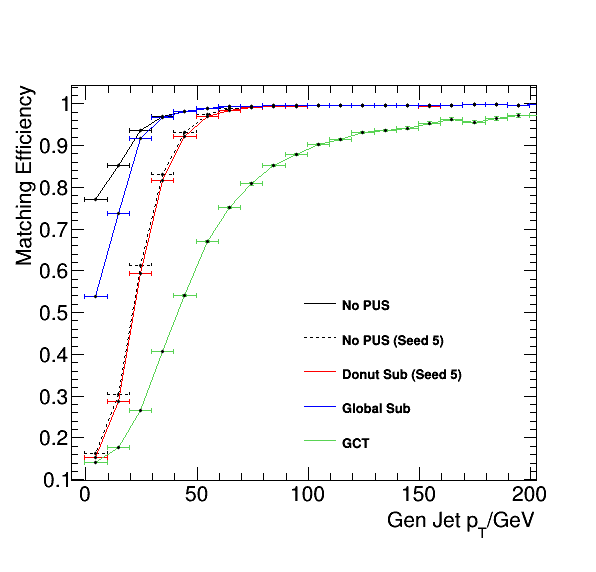
\includegraphics[width=0.6\linewidth]{performance/matchingeff_alljet}
	\end{center}
	\caption{The efficiency with which a Gen jet has a corresponding L1 jet within a radius, $R=0.5$. This is carried out for all Gen jets in 70~000 $t\bar{t}$ events.}
	\label{fig:matchingeff}
\end{figure}
\\\\
\noindent To characterise the energy performance of the L1 jets, turnon curves are plotted in Fig.~\ref{fig:turnons}. These are made by matching the Gen jets to L1 jets, requiring $\Delta R<0.5$ and taking the matched Gen $p_T$ distribution without a cut on L1 jets and one with a cut on the L1 jets, then dividing the two histograms. The fourth leading jet of a $t\bar{t}$ sample is used as it displays the biggest discrepancy between algorithms. By $80$~GeV the PUS doesn't affect the resolution except for donut subtraction which appears to be over subtracting energy in a small number of cases.
\begin{figure}
	\begin{center}
		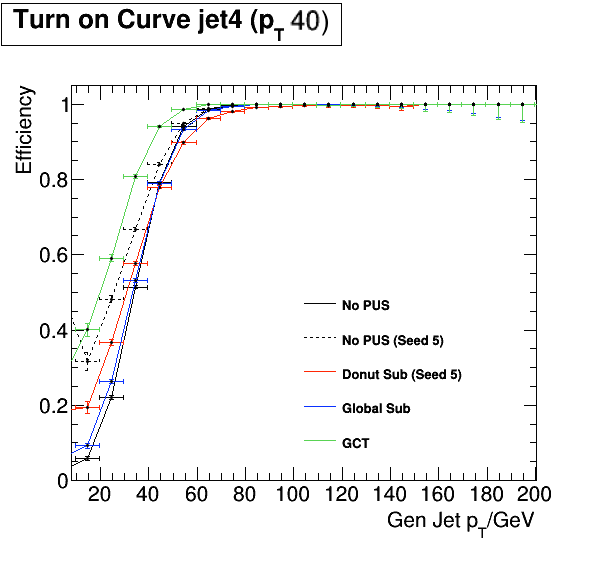
\includegraphics[width=0.5\linewidth]{performance/turnon_jet4_40}\put(-42,203){(a)}
		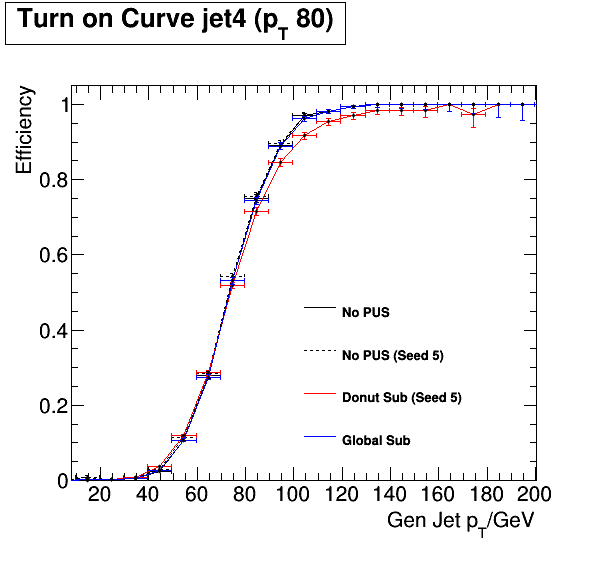
\includegraphics[width=0.5\linewidth]{performance/turnon_jet4_80}\put(-42,203){(b)}
	\end{center}
	\caption{The proportion of remaining Gen jets matched to fourth leading L1 jets after performing a cut on L1 of (a) 40GeV, (b) 80GeV.}
	\label{fig:turnons}
\end{figure}
%turnons - how energy matched to gen - gct bad
\\\\
\noindent To measure the performance of the PUS algorithms removing soft QCD PU jets, the rate against the number of interactions is plotted for the zero bias sample for a representative $p_T$ cut of $30$~GeV, Fig.~\ref{fig:ratenvtx}. The PUS clearly lowers the dependence on the number of interactions and reduces the rate of jets passing the cut, it is performing as it should. It seems that the seed threshold is the most effective at killing soft QCD, with donut subtraction on top not making much difference. GCT jets are incredibly sensitive to PU, further motivating the trigger upgrade.
\begin{figure}
	\begin{center}
		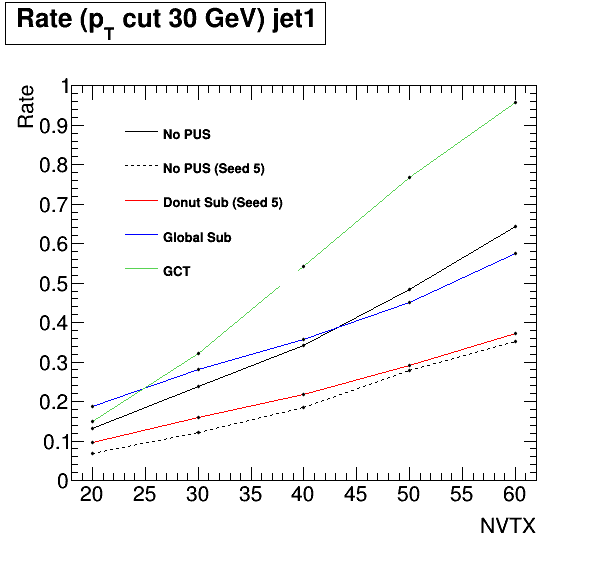
\includegraphics[width=0.5\linewidth]{performance/ratenvtx_neutrino_jet1}\put(-42,203){(a)}
		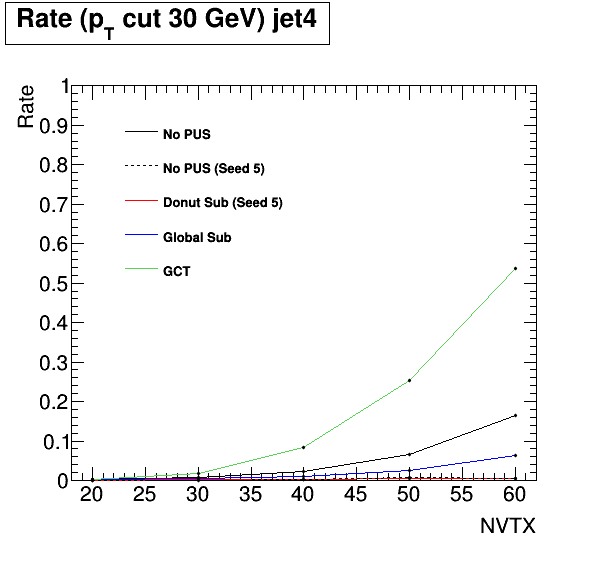
\includegraphics[width=0.5\linewidth]{performance/ratenvtx_neutrino_jet4}\put(-42,203){(b)}
	\end{center}
	\caption{The relative rate of L1 jets with $p_T>30$~GeV after PUS for the leading jet, (a), and fourth leading jet, (b), for $70 000$ zero bias events as a function of the number of interactions (NVTX)}
	\label{fig:ratenvtx}
\end{figure}
%level of soft qcd pileup subtraction- rate vs nvtx
\\\\
\noindent To ensure that the PUS algorithms are not too aggressive, efficiency is plotted against the rate from a zero bias sample given a certain $p_T$ cut. Efficiency is defined as the fraction of events with a lead Gen jet of $p_T>50$~GeV that have a lead L1 jet that is matched to a Gen jet ($\Delta R<0.5$). Ideally the efficiency remains close to one while reducing as much rate as possible. It can be seen in Figure~\ref{fig:rateeff} that for the leading jet very good efficiency is retained in all cases, with the fluctuations in donut subtraction affecting it.
\begin{figure}
	\begin{center}
		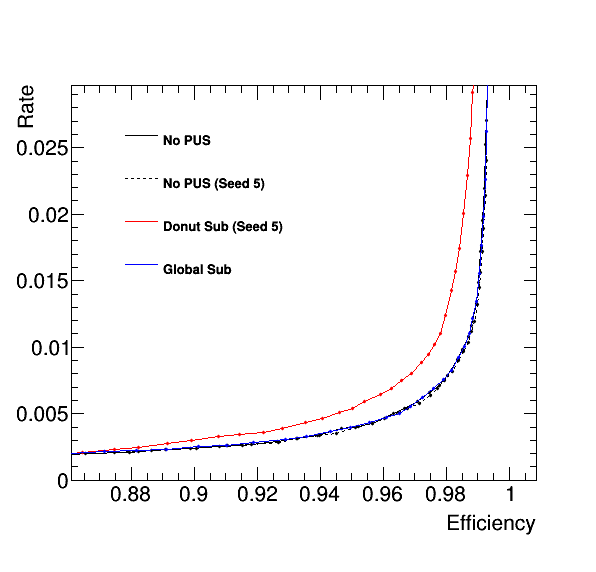
\includegraphics[width=0.6\linewidth]{performance/jet1RateEff}
	\end{center}
	\caption{The normalised rate against efficiency for various PUS schemes. Efficiency is defined as the fraction of events with a lead Gen jet of $p_T>50$~GeV that have a lead L1 jet that is matched to a Gen jet (dR<0.5). Based on a $t\bar{t}$ and zero bias sample.}
	\label{fig:rateeff}
\end{figure}
%\begin{figure}
%	\begin{center}
%		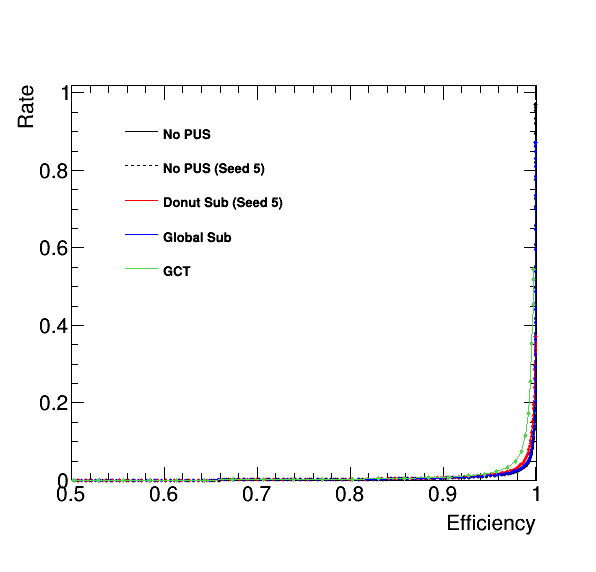
\includegraphics[width=0.5\linewidth]{performance/rateseff_jet1}\put(-42,203){(a)}
%		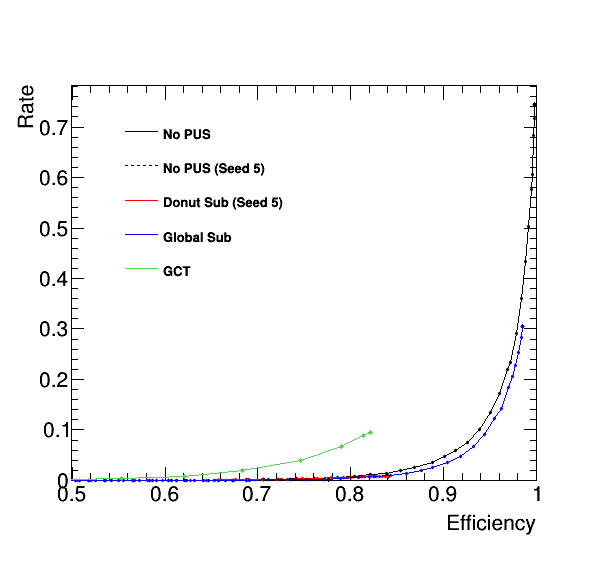
\includegraphics[width=0.5\linewidth]{performance/rateseff_jet4}\put(-42,203){(b)}
% 	\end{center}
%	\caption{Given a particular $p_T$ cut on a level 1 jet the proportion of remaining leading, (a), and fourth %leading, (b), jets is plotted for a zero bias sample against a $t\bar{t}$ sample. The rate is represented by the %zero bias sample and the efficiency by the $t\bar{t}$}
%	\label{fig:rateeff}
%\end{figure}
%maintaining signal- rateseff
\\\\
\noindent The other purpose of PUS is to correct the energy of L1 jets contaminated with PU. The resolution of the jets as compared to Gen is defined as $\frac{p_T^{L1}-p_T^{Gen}}{p_T^{Gen}}$, being zero for perfect agreement. The PUS should act to remove the dependence of the resolution on the number of interactions in an event. In Figure~\ref{fig:resolution} it can be seen that the donut and global $\rho$ subtraction do flatten out the resolution for a representative bin of $p_T$ and $\eta$, whereas the seed on its own does not. 
\begin{figure}
	\begin{center}
		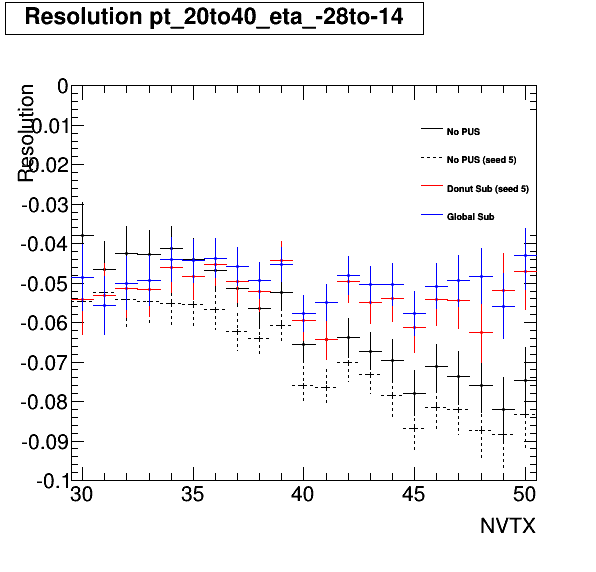
\includegraphics[width=0.6\linewidth]{performance/pt_20to40_eta_-28to-14}
	\end{center}
	\caption{The resolution of L1 jets with $20<p_T<40$~GeV and with $-3<\eta<-1.2$ as a function of the number of interactions (NVTX)}
	\label{fig:resolution}
\end{figure}
%correcting hard jets- response
\\\\
\noindent As a final performance test, the $H_T$ and $\cancel{H}_T$ as defined in Section~\ref{sec:alphaT} are plotted. If the PUS is too aggressive the $H_T$ will be too low when compared to Gen, or too high if it under subtracts. Figure~\ref{fig:htmht} shows that jets with a seed threshold most closely reproduce the $H_T$. Overall the PUS methods are under subtracting, however. The PUS does not improve the $\cancel{H}_T$ distribution, this is expected in the case that PU is distributed evenly.
\begin{figure}
	\begin{center}
		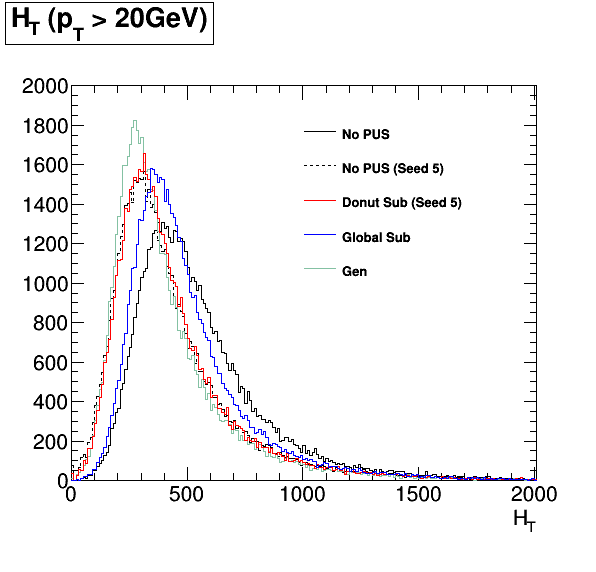
\includegraphics[width=0.5\linewidth]{performance/ht_ttbar}\put(-42,203){(a)}
		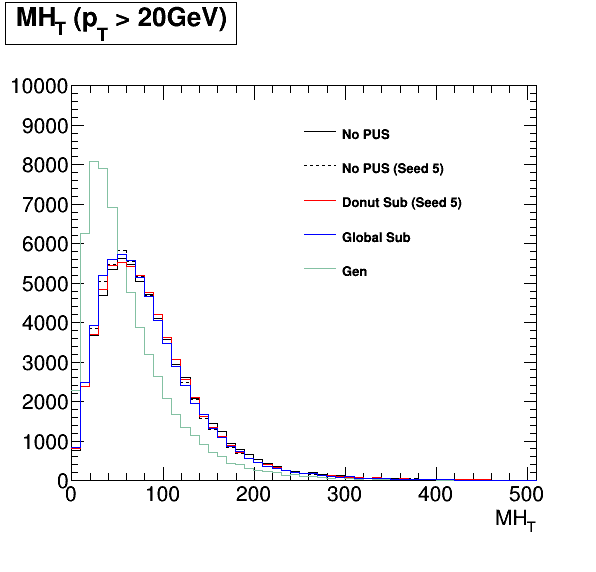
\includegraphics[width=0.5\linewidth]{performance/mht_ttbar}\put(-42,203){(b)}
	\end{center}
	\caption{(a) The distribution of the total energy of jets in each event ($H_T$). (b) The distribution of the missing momentum of jets in an event ($\cancel{H}_T$).}
	\label{fig:htmht}
\end{figure}
%not killing important jets- ht mht
\\\\
\noindent The proposed Stage 2 jet algorithm performs well with respect to the previous GCT algorithm. With the introduction of PUS, the more challenging conditions at 13TeV in Run 2 can start to be tamed. The rate of reconstructed jets can be reduced without sacrificing too much efficiency. Global subtraction and donut subtraction both help to remove the dependence of the energy of signal jets on PU. Due to fluctuations in the donut subtraction, the efficiency takes a hit, but it is better at reproducing the $H_T$ distribution than global $\rho$. This is just the beginning of the investigation of PUS for L1 jets, further investigation is required to optimise the parameters used and compare to other PUS schemes.
%conclusion